\documentclass{article}

\usepackage{amsmath}
\usepackage{tikz}

\begin{document}

    \begin{center}
        \textbf{BILANGAN KOMPLEKS}
    \end{center}

    Bilangan Kompleks adalah bilangan yang dapat direpresentasikan sebagai \( x + iy \), dimana $x$ dan $y$ adalah bilangan real ($R$) dan $i$ adalah suatu bilangan imaginer dimana \( i = \sqrt{-1} \) dan \( i^2 = -1 \).\\

    Bilangan Kompleks biasanya ditulis dalam bentuk:
    \begin{align}
        x = x + iy
    \end{align}

    \>dimana,\\
    - $x$ adalah bagian $Re(z)$, dan\\
    - $y$ adalah bagian $Im(z)$.\\

    Contoh:
    \begin{align}
        z & = 6 + \sqrt{-16} 
        \nonumber\\
        & = 6 + \sqrt{-1} \times \sqrt{16}
        \nonumber\\
        & = 6 + i \times 4
        \nonumber\\
        & = 6 + 4i
    \end{align}

    maka:\\
    -   $Re(z) = 6$, dan\\
    -   $Im(z) = 4$.\\\\

    \begin{center}
        \textbf{Notasi Bilangan Kompleks}
    \end{center}
    
    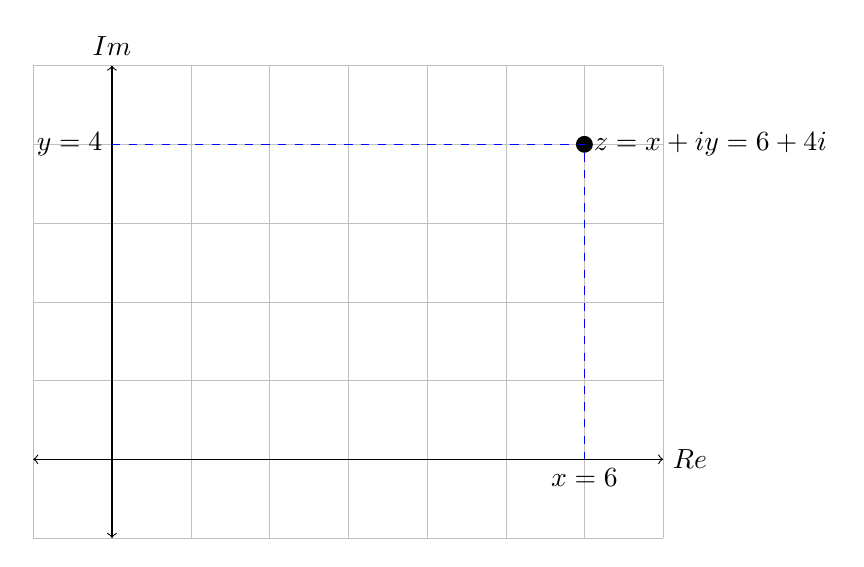
\begin{tikzpicture}
        \draw [ultra thin, lightgray] (-1,-1) grid (7,5);
        \draw [<->] (-1, 0) -- (7, 0) node[right] {$Re$};
        \draw [<->] (0, -1) -- (0, 5) node[above] {$Im$};
        \draw [black, fill = black] (6,4) circle [radius = 1 mm]
            node[black, right] {$ z = x + iy = 6 + 4i $};
        \draw [blue, dashed] (0,4) node[black, left] {$ y = 4 $}
            -| (6,0) node[black, below] {$ x = 6 $};
    \end{tikzpicture}

\end{document}